\section{Applications}

Based on our generalization error framework, we now have a rigorous way to analyze WS settings with misspecification. We examine two practical applications of our theoretical results under three settings---well-specified, misspecified, and corrected.
\begin{itemize}
    % \item \textbf{Correcting for misspecification:} for the weakly labeled data setting, we propose a simple algorithm improving over random selection of triplets $\lf_i, \lf_j, \lf_k$ that removes the error term $\varepsilon_{\max} \left(\frac{c_1 d}{m} + \frac{c_2}{\sqrt{n_U}} + \frac{c_3}{n_U}\right)$ given that $m$ is large and $d$ is $o(m^2)$.
    \item \textbf{Understanding the value of labeled data:} we address our motivating question about the value of labeled data–is a few labeled samples or many weakly labeled samples better? This decision depends on the misspecification parameters ($d$, $\varepsilon_{\max}$), and $n_U$ versus $n_L$.
    \item \textbf{Combining labeled and unlabeled data:} we show how simple linear combinations of the estimators can improve generalization error bounds over using one or the other. Then, we suggest a James-Stein type estimator from~\cite{GreenStrawderman2001}, which combines an unbiased estimator with biased information, to easily determine the weights of the linear combination. %Based on our misspecification analysis, we show that this estimator offers a \textcolor{red}{X} improvement in generalization error. 
\end{itemize}

%In this section, we discuss these two consequences of our framework theoretically. In section \ref{sec:exp}, we verify them on synthetic and real data.


\subsection{Understanding the value of labeled data}
We use our analysis from section \ref{subsec:scaling} to develop a criterion for deciding between $n_L$ labeled points and $n_U$ weakly labeled points. Compute
\[\alpha(n_U) = \min_{n_L \in \mathbb{N}} \text{ s. t. } R_L^{\mathrm{excess}}(n_L) \le R_U^{\mathrm{excess}}(n_U),\]
%where $U^{\text{unlabeled}}, U^{\text{labeled}}$ are the upper bounds on the excess generalization error for unlabeled and labeled data, respectively.
and define
%\begin{align}
$V(n_U) = {n_U}/\alpha(n_U)$
%\end{align}
to be the \textit{data value ratio}. The intuitive idea here is to compare, for each amount of weakly labeled data $n_U$, what factor less labeled data we would require to produce an equivalent error bound. We consider an approximation of the data value ratio $\widetilde{V}(n_U)$ based on our upper bounds for $R_U$ and $R_L$ in Theorems \ref{thm:labeled} and \ref{thm:unlabeled}. We examine the differences in $\widetilde{V}(n_U)$ for our three aforementioned settings:
\begin{itemize}
    \item Well-specified setting: comparing excess risk when $d = 0$ and $\varepsilon_{\max} = 0$ reduces to examining $\frac{m}{2n_L}$ and $\frac{c_4 m}{n_U}$. Thus $\widetilde{V}(n_U) = 2c_4$ and our framework suggests that labeled data is only a constant factor more beneficial than weakly labeled data.
    \item Misspecified setting: $V(n_U)$ in this case will capture the tradeoff between $\frac{m}{2n_L}$ and $\B_{\mathrm{est}} + \frac{c_4 m }{n_U}$. We find that $\widetilde{V}(n_U) = 2 \varepsilon_{\max} \left(\frac{c_1 dn_U}{m} + \frac{c_2 \sqrt{n_U}}{m} + +\frac{c_3 d}{m^2} \right) + 2 c_4$. That is, the value of labeled data \textit{increases linearly in the amount of unlabeled data and misspecification} due to the standing bias in the generalization error for the weakly labeled data case.  
    \item Corrected setting: under our conditions from Proposition \ref{prop:medians}, we examine the difference between $\frac{m}{2n_L}$ and $ c_\rho m \rho_{n_
    U}$, and thus $\widetilde{V}(n_U) = 2n_U c_{\rho} \rho_{n_U}$. Since $\rho_{n_U}$ converges to $0$, $\widetilde{V}(n_U)$ is sublinear in $n_U$, showing that the \textit{corrected model reduces the value of labeled data.}
\end{itemize}

\paragraph{Synthetic Experiments} We measure $V(n)$ in well-specified, misspecified and corrected settings on synthetic data with the same setup as previously discussed. 
%We expect three principles to hold: first, for a well-specified model, the data value ratio is small and roughly constant, second, the ratio scales with misspecification and finally, the ratio is smaller for a corrected model than for a misspecified model. \bcw{Get rid of this sentence?} We also expect that our theoretical ratio produces a reasonable estimate of the empirical value, in particular one that tracks the scaling of the misspecification level. 
We present the results in \autoref{fig:data_value_ratio}. In the well-specified case ($d = 0$), $V(n)$ is small (less than $5$) and roughly constant across $n$. Under misspecification however, the data value ratio grows with both $d$ and $n$ albeit much more slowly for the corrected setting, aligning with our theoretical findings. 

\begin{figure}
    \centering
    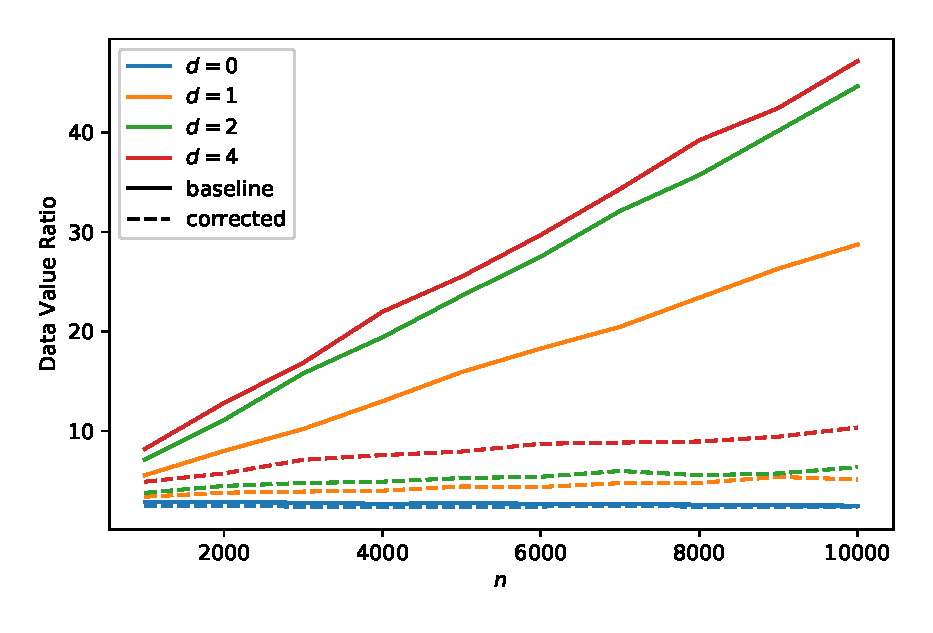
\includegraphics[width=.4\textwidth]{eps_figures/data_value_ratio_vs_n.eps}
    %
    \caption{Data value ratio vs. $n$, using both the baseline weak supervision model and the corrected model, which aggregates results over triplets using medians. Note that $d=0$ represents the well-specified setting. %We see that in the well-specified case ($d=0$) the data value ratio is small and roughly constant across $n$. Under misspecification, the data value ratio grows with $d$ for both the baseline and corrected models, but grows faster for baseline models, as reflected by our theoretical model.
    }
    \label{fig:data_value_ratio}
\end{figure}

%Based on Theorems \ref{thm:labeled} and \ref{thm:unlabeled}, we see that this ratio captures the tradeoff between $\varepsilon_{\max} \big(\frac{c_1 d}{m} + \frac{c_2 m}{\sqrt{n_U}} + \frac{c_3 m}{n_U} \big) + \frac{c_4 m}{n_U}$ and $\frac{m}{2n_L}$. In particular, %for a weakly labeled dataset to have a better generalization error, 
% we must have that $\alpha(n) = c\big(\frac{\varepsilon_{\max} n m^2}{m^2 - \varepsilon_{\max} d n}\big)^2$ for some constant $c$ and $n < \frac{m^2}{\varepsilon_{\max} d}$; when $n$ is too large, it is possible that no amount of unlabeled data can achieve the same generalization error due to the standing bias. Therefore, as any  one of $n, \varepsilon_{\max}$, or $d$ increases, the threshold for weakly labeled points becomes higher. On the other hand, if we were to ignore misspecification, we only require that $V(n) = 2c_4$ be a constant value, which as a criterion could lead to wrong decisions if the model is actually incorrect.
% We use our analysis from section \ref{subsec:scaling} to develop a criterion for deciding between $n_L$ labeled points and $n_U$ weakly labeled points. Let $n = n_L$, and then compute
% \[\alpha(n) = \min_{n_U \in \mathbb{N}} \text{ s. t. } U^{\text{unlabeled}}(n_U) \leq U^{\text{labeled}}(n),\]
% where $U^{\text{unlabeled}}, U^{\text{labeled}}$ are the upper bounds on the excess generalization error for unlabeled and labeled data, respectively.
%
% Then, the ratio
% %\begin{align}
% $V(n) = \alpha(n)/{n}$
% %\end{align}
% represents the value of labeled over weakly labeled data. The intuitive idea here is to compare, for each amount of labeled data $n$, what factor greater unlabeled data we would require to produce an equivalent error bound. 
% Based on Theorems \ref{thm:labeled} and \ref{thm:unlabeled}, we see that this ratio captures the tradeoff between $\varepsilon_{\max} \big(\frac{c_1 d}{m} + \frac{c_2 m}{\sqrt{n_U}} + \frac{c_3 m}{n_U} \big) + \frac{c_4 m}{n_U}$ and $\frac{m}{2n_L}$. In particular, %for a weakly labeled dataset to have a better generalization error, 
% we must have that $\alpha(n) = c\big(\frac{\varepsilon_{\max} n m^2}{m^2 - \varepsilon_{\max} d n}\big)^2$ for some constant $c$ and $n < \frac{m^2}{\varepsilon_{\max} d}$; when $n$ is too large, it is possible that no amount of unlabeled data can achieve the same generalization error due to the standing bias. Therefore, as any  one of $n, \varepsilon_{\max}$, or $d$ increases, the threshold for weakly labeled points becomes higher. On the other hand, if we were to ignore misspecification, we only require that $V(n) = 2c_4$ be a constant value, which as a criterion could lead to wrong decisions if the model is actually incorrect.

%Equivalently, we require that $d$ must be of order  $o\big(\frac{m^2}{\varepsilon_{\max}}\big(\frac{1}{n_L} - \frac{1}{\sqrt{n_U}}\big)\big)$ for a weakly labeled dataset to have better generalization error. 


%Therefore, when $d$ and $\varepsilon_{\max}$ are both small while $n_L$ is also small, $V(n)$ should suggest a reasonably-sized $n_U$ in order for an unlabeled dataset to yield higher performance. On the other hand, when there are many unmodeled dependencies and all of them are strong, $V(n)$ should be very large, suggesting that a small labeled dataset performs better.

\subsection{Combining labeled and unlabeled data}
While we now have a criterion to choose between datasets, how do we combine information from both? We examine ways to combine the accuracy parameters, namely $\widetilde{a}^U$ as defined in \eqref{eq:triplet} for weakly-labeled data and an equivalent $\widetilde{a}^L := \Ehat{\bm{\lf} Y}$ for labeled data. Recall that $\widetilde{a}^L$ is unbiased, while $\widetilde{a}^U$ is both biased and inconsistent. 

First, we consider a simple linear combination, $a^{\mathrm{lin}} = \alpha \widetilde{a}^U + (1 - \alpha) \widetilde{a}^L$ for some weight $\alpha \in [0, 1]$. Using our framework in \ref{thm:decomposition}, we can derive similar upper bounds on excess generalization error when the estimator is $a^{\mathrm{lin}}$. We summarize our findings across the three settings below. 
\begin{itemize}
    \item Well-specified setting: the upper bound on excess generalization error using $a^{\mathrm{lin}}$, ignoring $\B_I$ and lower order terms, is $\alpha^2 \frac{c_4 m}{n_U} + (1 - \alpha)^2 \frac{m}{2n_L}$. One can easily verify that there exists an $\alpha \in (0, 1)$ that minimizes this upper bound. Since $n_U$ is usually much larger than $n_L$, plugging in this optimal $\alpha$ shows that this new upper bound is roughly of the same order as the weakly-labeled case. \steve{Do you think it is sufficiently clear that the optimal $\alpha$ is independent of the specific run?}
    \item Misspecified setting: the upper bound is a cubic polynomial in $\alpha$. We find that the optimal $\alpha$ approaches $0$ more quickly as $n_L$ increases due to $\B_{\mathrm{est}}$ with standing bias. This suggests that a combined estimator can yield an upper bound much smaller than that for the weakly-labeled case.
    \item Corrected setting: the upper bound now consists of $\alpha^2 c_{\rho} m \rho_{n_U} + (1 - \alpha)^2 \frac{m}{2n_L}$. As a function of $\alpha$, this differs from the well-specified setting's expression only in constant coefficients, so this again suggests an optimal $\alpha \in (0, 1)$ and performance roughly similar to the weakly-labeled case.
\end{itemize}

% We produce an upper bound on excess generalization error from using $a^{\mathrm{lin}}$ similar to our results in Theorems \ref{thm:labeled} and \ref{thm:unlabeled}.
%\begin{align}
%    R_{\mathrm{lin}}^{\mathrm{excess}}(\alpha)\le & \varepsilon_{\max}\Big(\frac{c'_1 \alpha d }{m} + \frac{c'_2 \alpha^2 }{\sqrt{n_U}} + \frac{c'_3 \alpha^3 d}{m n_U} \\
%    &+ \frac{\alpha (1 - \alpha)^2 c'_5 d}{m n_L} \Big) + \frac{c'_4 \alpha^2 m}{n_U} \nonumber \\
%    &+ \frac{(1 - \alpha)^2 m}{2n_L} + \B_I + o(1/n_L), \nonumber
%\end{align}
% \mayee{need to change into structure that parallels 5.1. Basically we say that for misspecified case, gen err is cubic polynomial in $\alpha$ and suggests that no local minimum in $(0, 1)$ unless $n_L$ is small (i.e. we usually just want to use labeled data, unlabeled is not good). For well-specified and corrected case, gen err is $\alpha^2 \Var{U}{n_U} + (1 - \alpha)^2 \Var{L}{n_L}$, and this yields an $\alpha \in (0, 1)$ given our variance constants are different enough, i.e. labeled data value is ``reduced''}.

%where $c'$ are scaled from the constants used in Theorems \ref{thm:labeled} and \ref{thm:unlabeled}. It is possible that this upper bound is minimized using some $\alpha \in (0, 1)$, especially when $n_L$ is small, which would suggest that a simple linear combination of the two estimators does better than using either one of them. We test a range of $\alpha$ on our synthetic datasets to confirm this.

%From Lemma \ref{lemma:accuracy_bias}, we see that $\widetilde{a}_i^U$ is biased while $\widetilde{a}_i^L$ is not. At first glance, it would seem that we should simply rely on the unbiased estimator---however, as known from Stein's phenomenon, this is not necessarily the right approach.
In practice, we do not know the exact $\alpha$ that optimizes generalization error. However, there is vast literature on combined estimators that dominate the MLE estimator $\widetilde{a}^L$. In particular, we suggest using an approach from~\cite{GreenStrawderman2001}, who propose a way of combining an unbiased estimator with biased information, and evaluate this combined estimator empirically. % the following combined estimator:
%\begin{align}
%    \bar{a} := \widetilde{a}^U + \bigg(1 - \frac{r}{(\widetilde{a}^L - \widetilde{a}^U)^T \Sigma^{-1} (\widetilde{a}^L - \widetilde{a}^U)} \bigg)_{\mathclap{+}} (\widetilde{a}^L - \widetilde{a}^U),
%\end{align}
%\begin{align}
%    \bar{a}_i := \widetilde{a}_i^L - \frac{(m - 2) }{n_L \|\widetilde{a}_i^L - \widetilde{a}_i^U \|_2^2} (\widetilde{a}_i^L - \widetilde{a}_i^U)
%\end{align}
%where $\Sigma = \Cov(\widetilde{a}^L)$, and $r \in [0, 2(m - 2)]$.  
%They show that this estimator dominates $\widetilde{a}^L$ when the unbiased estimator is Gaussian and its covariance is known. However, since we can only estimate the covariance matrix, we replace $\Sigma$ with an empirical estimate $\hat{\Sigma}$. Moreover, since $\widetilde{a}^L$ is only Gaussian asymptotically, we do not provide theoretical guarantees on $\bar{a}$ but instead empirically validate its performance. \todo{story here: this estimator builds upon naive linear combination (just how to set the $\alpha$) }

%This estimator has been proven to dominate the unbiased $\widetilde{a}^L$ when the true covariance matrix $\Sigma$ is known, even when $\widetilde{a}^U$ is very biased \steve{we don't have normality though, right?}. %In particular, \cite{GreenStrawderman1991} show that
%Using their equation 2.5, it is true that
%\begin{align}
%    &\E{}{\|\bar{a} - a \|_2^2} \le m Var(\widetilde{a}_i^L) - \nonumber \\
%    &\frac{Var(\widetilde{a}_i^L)^2 (m - 2)^2}{\|\E{}{\widetilde{a}^U} - a \|_2^2 + (m - 2)(\sqrt{Var(\widetilde{a}_i^L)} + Var(\widetilde{a}_i^U))} \nonumber
%\end{align}

%which, when plugged into our decomposition framework in Theorem \ref{thm:decomposition}, gives us a better generalization error \todo{be more precise here.}

%We now show that the label model generalization error using $\bar{a}$ is better than that using either $\widetilde{a}_i^U$ or $\widetilde{a}_i^L$. \todo{plug above eqn into thm 1 type bound}.

\paragraph{Synthetic Experiments} We investigate the empirical performance of estimators which combine labeled and unlabeled data in well-specified, misspecified and corrected settings. We measure both the error when using the optimal weight $\alpha$ and the more practical approach of \cite{GreenStrawderman2001}. We fix $n_U=1000$ and vary $n_L$ across a range of smaller values, in alignment with the assumption that many more unlabeled than labeled points are typically available. Our results are in Figure \ref{fig:combined}. In the well-specified setting, the combined estimators perform roughly the same as just $\widetilde{a}^U$; matching up with our theoretical observations for large $n_U$. In the misspecified setting, both combined estimators result in much lower excess risk than either estimator individually, and as $n_L$ increases, the labeled estimator curve approaches those of the combined estimators, suggesting that the weight on $\widetilde{a}^L$ increases as more labeled data becomes available. Lastly, in the corrected setting both combined estimators perform better than $\widetilde{a}^U$, but not by much.
%suggesting that there is a standing bias present in the former case that makes combining with labeled data more helpful.
%The approach of \cite{GreenStrawderman2001} does not consistently outperform the unlabeled only approach in the well-specified case, where the unlabeled estimator is unbiased. However, it significantly outperforms either individual approach in the misspecified case and outperforms either individual approach in the corrected case. 
The weights $\alpha$ are reported in the Appendix. The optimal weights for the well-specified and corrected settings are higher (i.e. more weight on the unlabeled estimator) than the misspecified setting, and these weights decrease with $n_L$.

%We expect that in the well-specified case, the combined estimators won't significantly outperform the unlabeled estimator. On the other hand, under misspecification, we expect the combined estimators, which account for the standing bias of unlabeled data, to provide a superior estimate to either individual estimator. Finally, for the corrected case, we expect more modest improvements from combining labeled and unlabeled data, similarly to the well-specified case. As the estimator proposed by \cite{GreenStrawderman1991} assumes that the unlabeled estimator is biased, we expect it to perform the best in the misspecified case compared to the optimal combined estimator. We present the results in \autoref{fig:combined}.

% We further expect the James-Stein-type estimator to perform better under misspecification where the unlabeled estimator is biased and the simple linear combination to perform better for well-specified models. Results in \autoref{fig:combined}.

\begin{figure}
    \centering
    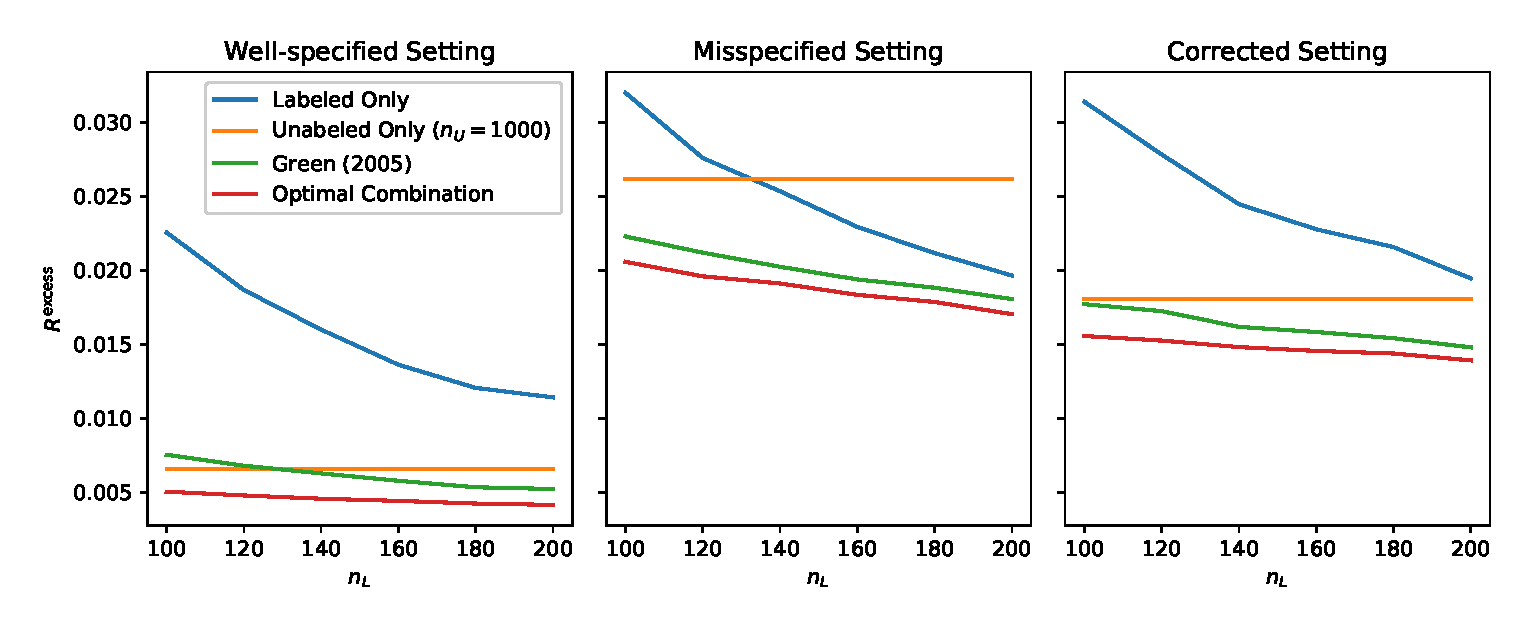
\includegraphics[width=.48\textwidth]{eps_figures/combined.eps}
    %
    \caption{Excess generalization error for an optimally weighted combination of labeled and unlabeled estimators, and a combination weighted according to \cite{GreenStrawderman2001} across the well-specified (left), misspecified (center), and corrected (right) settings. %The approach of \cite{GreenStrawderman2001} does not consistently outperform the unlabeled only approach in the well-specified case, where the unlabeled estimator is unbiased. However, it significantly outperforms either individual approach in the misspecified case and outperforms either individual approach in the corrected case. The combination weights are reported in the \todo{Appendix}. Broadly, the optimal weights for the well-specified and corrected settings are higher than the misspecified setting, and these weights decrease with $n_L$.
    }
    \label{fig:combined}
\end{figure}